A contactless bank card has no battery: a flat coil in the card ($L = \LcO$) picks up the field of the reader, at \fzO. With a capacitor, the coil forms a parallel resonant circuit tuned to that frequency; the chip acts as the resistor. The graph shows the measured impedance of the circuit.

\begin{center}
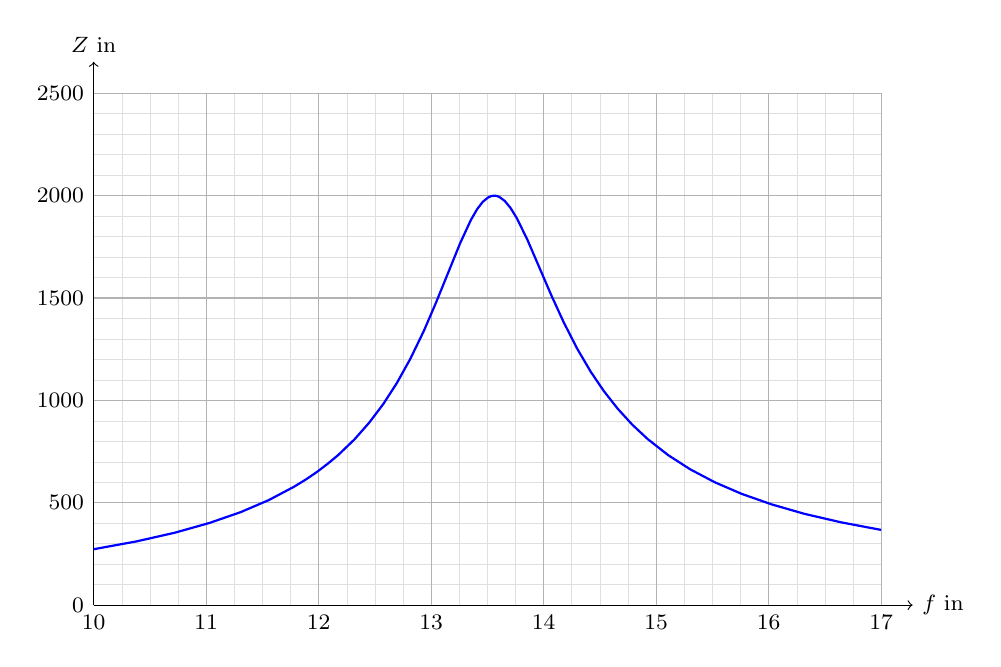
\begin{tikzpicture}[font=\footnotesize]
 \draw[gray!25, very thin] (0.357,0) -- (0.357,6.500) (0.714,0) -- (0.714,6.500) (1.071,0) -- (1.071,6.500) (1.786,0) -- (1.786,6.500) (2.143,0) -- (2.143,6.500) (2.500,0) -- (2.500,6.500) (3.214,0) -- (3.214,6.500) (3.571,0) -- (3.571,6.500) (3.929,0) -- (3.929,6.500) (4.643,0) -- (4.643,6.500) (5.000,0) -- (5.000,6.500) (5.357,0) -- (5.357,6.500) (6.071,0) -- (6.071,6.500) (6.429,0) -- (6.429,6.500) (6.786,0) -- (6.786,6.500) (7.500,0) -- (7.500,6.500) (7.857,0) -- (7.857,6.500) (8.214,0) -- (8.214,6.500) (8.929,0) -- (8.929,6.500) (9.286,0) -- (9.286,6.500) (9.643,0) -- (9.643,6.500);
 \draw[gray!25, very thin] (0,0.260) -- (10.000,0.260) (0,0.520) -- (10.000,0.520) (0,0.780) -- (10.000,0.780) (0,1.040) -- (10.000,1.040) (0,1.560) -- (10.000,1.560) (0,1.820) -- (10.000,1.820) (0,2.080) -- (10.000,2.080) (0,2.340) -- (10.000,2.340) (0,2.860) -- (10.000,2.860) (0,3.120) -- (10.000,3.120) (0,3.380) -- (10.000,3.380) (0,3.640) -- (10.000,3.640) (0,4.160) -- (10.000,4.160) (0,4.420) -- (10.000,4.420) (0,4.680) -- (10.000,4.680) (0,4.940) -- (10.000,4.940) (0,5.460) -- (10.000,5.460) (0,5.720) -- (10.000,5.720) (0,5.980) -- (10.000,5.980) (0,6.240) -- (10.000,6.240);
 \draw[gray!60, thin] (0.000,0) -- (0.000,6.500) (1.429,0) -- (1.429,6.500) (2.857,0) -- (2.857,6.500) (4.286,0) -- (4.286,6.500) (5.714,0) -- (5.714,6.500) (7.143,0) -- (7.143,6.500) (8.571,0) -- (8.571,6.500) (10.000,0) -- (10.000,6.500);
 \draw[gray!60, thin] (0,0.000) -- (10.000,0.000) (0,1.300) -- (10.000,1.300) (0,2.600) -- (10.000,2.600) (0,3.900) -- (10.000,3.900) (0,5.200) -- (10.000,5.200) (0,6.500) -- (10.000,6.500);
 \node[below] at (0.000,0) {10};
 \node[below] at (1.429,0) {11};
 \node[below] at (2.857,0) {12};
 \node[below] at (4.286,0) {13};
 \node[below] at (5.714,0) {14};
 \node[below] at (7.143,0) {15};
 \node[below] at (8.571,0) {16};
 \node[below] at (10.000,0) {17};
 \node[left] at (0,0.000) {0};
 \node[left] at (0,1.300) {500};
 \node[left] at (0,2.600) {1000};
 \node[left] at (0,3.900) {1500};
 \node[left] at (0,5.200) {2000};
 \node[left] at (0,6.500) {2500};
 \draw[->] (0,0) -- (10.400,0) node[right] {$f$ in \si{\mega\hertz}};
 \draw[->] (0,0) -- (0,6.900) node[above] {$Z$ in \si{\ohm}};
 \draw[thick, blue] plot coordinates {(0.000,0.710) (0.543,0.809) (1.032,0.920) (1.472,1.044) (1.867,1.181) (2.224,1.334) (2.547,1.505) (2.697,1.597) (2.839,1.694) (2.975,1.798) (3.106,1.907) (3.311,2.104) (3.501,2.320) (3.679,2.556) (3.849,2.819) (4.021,3.128) (4.191,3.479) (4.347,3.841) (4.654,4.597) (4.789,4.889) (4.869,5.028) (4.942,5.123) (5.013,5.180) (5.048,5.194) (5.083,5.200) (5.116,5.197) (5.151,5.184) (5.221,5.132) (5.294,5.043) (5.374,4.913) (5.509,4.637) (5.814,3.929) (5.971,3.587) (6.141,3.255) (6.313,2.962) (6.478,2.719) (6.653,2.496) (6.838,2.293) (7.036,2.108) (7.295,1.905) (7.578,1.723) (7.890,1.559) (8.231,1.412) (8.610,1.279) (9.027,1.159) (9.488,1.052) (10.000,0.955)};
\end{tikzpicture}
\end{center}

\begin{abcliste}
\abc Which capacitance $C$ is built into the card?
\abc Read the bandwidth $\Delta f$, the width of the peak where $Z = Z_\mathrm{max}/\sqrt{2}$.
\abc What is the quality factor $Q = f_0/\Delta f$?
\end{abcliste}
